% Print
\documentclass[DIV=15,headinclude=true]{scrreprt}

%Packages, die für die deutsche Sprache erforderlich sind
\usepackage[utf8]{inputenc}
\usepackage[T1]{fontenc}
\usepackage{lmodern}
\usepackage[ngerman]{babel}
\usepackage{csquotes}

%Packages für Graphik
\usepackage[]{graphicx}
\graphicspath{{figures/}}

\usepackage{amsmath}

%BibLaTex
\usepackage[backend=biber]{biblatex}
\addbibresource{literature/bibliography.bib} 

%Package, damit Bibtex-URL klappt
\usepackage[pdfusetitle]{hyperref}
\usepackage{url}

%Noch schönere Typographie
\usepackage{microtype}

\usepackage{todonotes}
\usepackage{booktabs}
\usepackage{tabulary}
\usepackage{multirow, makecell}

\usepackage{pdflscape}
\usepackage{afterpage}

\usepackage{multicol}

%Kästen
\usepackage{framed}

%%%%% BEGINN KOPF- UND FUẞZEILE %%%%%
\usepackage[headsepline,footsepline]{scrlayer-scrpage}
\usepackage{graphicx}
\pagestyle{scrheadings}
\ohead{\includegraphics[height=1cm]{figures/bluemarble}}
\chead{\headmark}
\automark{section}
%\ihead{\includegraphics[height=1cm]{bluemarble.jpg}}
\ifoot{\csname @title\endcsname}\cfoot{\pagemark}
\ofoot{\today}
%%%%% ENDE KOPF- UND FUẞZEILE %%%%%

\begin{document}
%%%%% BEGINN TITEL %%%%%
\title{Projektaufgabe und Bewertungskriterien}
\subtitle{Entwicklungsmethoden für nachhaltige Produkte}
\author{EnWiNaP-Team}
\maketitle
%%%%% ENDE TITEL %%%%%

%%%%% BEGINN FRONT MATTER %%%%%
\chapter*{Zusammenfassung}

In diesem Dokument sollten die meisten Informationen enthalten sein, die ihr benötigt, um eure Prüfungsleistung im Modul "`Entwicklungsmethoden für nachhaltige Produkte"' zu erbringen. Es gliedert sich in jeweils einen Teil zur Aufgabenstellung und einen Teil zu den Bewertungskriterien für die jeweilige Prüfungskomponente.


\tableofcontents
%%%%% ENDE FRONT MATTER %%%%%


%%%%% BEGINN INHALT %%%%%

\chapter{Basisdaten}

Die Veranstaltung ist als Portfolioprüfung\footnote{Rahmenbedingungen:
	\href{https://www.tu-berlin.de/asv/menue/gremien/kommissionen_des_as/hinweise_zur_allgstupo/hinweise_zu_portfoliopruefungen/}{\underline{hier}}}
konzipiert. Tabelle \ref{tab:zusammensetzung} zeigt die
Zusammensetzung der Gesamtnote auf die einzelnen Teilleistungen.

Die Note setzt sich als Portfolioprüfung zusammen aus den Prüfungsleistungen Lernjournal (Abschnitt \ref{lernjournal}), Projektbericht (Abschnitt \ref{projektbericht}) und Präsentation (Abschnitt \ref{präsentation}).

Zur Zuordnung der Portfoliopunkte zu den Noten kommt der
\enquote{Notenschlüssel 3} der Fakultät IV zur Anwendung, wie in Tabelle
\ref{tab:notenschluessel} gezeigt. Dieser
Notenschlüssel ist \enquote{großzügiger} als die üblicherweise an der
Fakultät V verwendeten. Wir wollen eine Lehrveranstaltung, in der
\enquote{sehr gut} nicht \enquote{fehlerfrei} bedeuten muss und wir
nicht eine Korrektur für die Punkte machen und eine, in der wir alle
Fehler aufzählen, die uns zwar aufgefallen sind aber für die wir keine
Punkte abziehen können, weil sonst die Note zu schlecht wird.
Studierende sollten also damit rechnen, das die Punktzahlen der
Teilleistungen schlechter als gewohnt ausfallen, die Noten jedoch nicht.

\begin{table}[!b]
	\begin{minipage}{.5\linewidth}
		\caption{Zusammensetzung der Gesamtnote}
		\begin{center}
			\label{tab:zusammensetzung}
			\begin{tabular}{llr}
				\toprule
				Name           & Typ         & Gewichtung \\
				\midrule
				Lernjournal    & individuell & 40 \%      \\
				Präsentation   & Gruppe      & 20 \%      \\
				Projektbericht & Gruppe      & 40 \%      \\
				\bottomrule
			\end{tabular}

		\end{center}
	\end{minipage}%
	\begin{minipage}{.5\linewidth}
		\caption{Notenschlüssel}
		\label{tab:notenschluessel}
		\begin{center}
			\begin{tabular}{lr}
				\toprule
				Punktzahl   & Note \\
				\midrule
				Punktzahl   & Note \\
				\(\geq\) 85 & 1,0  \\
				\(\geq\) 80 & 1,3  \\
				\(\geq\) 75 & 1,7  \\
				\(\geq\) 70 & 2,0  \\
				\(\geq\) 65 & 2,3  \\
				\(\geq\) 60 & 2,7  \\
				\(\geq\) 55 & 3,0  \\
				\(\geq\) 50 & 3,3  \\
				\(\geq\) 45 & 3,7  \\
				\(\geq\) 40 & 4,0  \\
				\(<\) 40    & 5,0  \\
				\bottomrule
			\end{tabular}
		\end{center}

	\end{minipage}
\end{table}







\chapter{Lernjournal}
\label{lernjournal}

\begin{framed}
Dir Lernjournalsbewertung wird blind durchgeführt, d.\ h. die Bewertenden kennen die Identität der Studierenden nicht. Aus diesem Grund darf die Matrikelnummmer sowie der Name \emph{nicht} im Dokument enthalten sein. Zur Identifizierung ist ein Deckname anzugeben, der nach der Prüfungsanmeldung zugeteilt wird.
\end{framed}


\section{Aufgabenstellung}

\emph{Ziel} des Lernjournals ist es, sich mit den vermittelten Inhalten
selbstständig erneut auseinanderzusetzen und sie in einem sorgfältig
erstellten Dokument aufzubereiten. Neben der Reproduktion sollen hier
auch eigene Einschätzungen und Interpretationen der Inhalte vermerkt
werden. Dabei soll sich die \underline{Reproduktion der Inhalte auf ein Minimum
	beschränken} (ca. 10-25\%) und die Reflexion der Inhalte der Schwerpunkt
(75-90\%) sein. Reflexion meint hier das Nachdenken über Zusammenhänge,
die nicht unmittelbar gegeben sind.

\emph{Formell} werden keine umfangreichen Anforderungen gestellt. Eine
\enquote{wissenschaftliche} Form (z.~B. so wie dieses Dokument +
Quellen) ist genauso akzeptabel wie eine kreativere Auseinandersetzung
mit Mindmaps, Zeichnungen und viel buntem Papier. Man sollte jedoch -- gerade wenn man das Format des wissenschaftlichen Berichts wählt -- den formellen Anforderungen des gewählten Formats folgen. Die Abgabe kann
physisch oder elektronisch erfolgen.

Wir erwarten einen \emph{Umfang} von ein bis zwei A4-Seiten (oder dem
Äquivalent dazu in anderen Formaten) für jeden Themenblock. Eine Überschreitung dieses Richtwerts durch zu hohe Reproduktionsanteile, Füllwörtern und inhaltslose Textpassagen führt zu Punktabzug.

\section{Bewertungskriterien}

Unten einige Grundlegende Gedanken, die exakte Bepunktung ist in
Tabelle \ref{tab:lernjournal} zu sehen. Die Berechnung der Portfoliopunkte für das Lernjournal erfolgt entsprechend der folgenden Formel.

\begin{equation*}
	\text{Portfoliopunkte} = 40 \times \frac{\text{Vollständigkeit}}{10} \times \frac{\text{Reflektion} \times 2 + \text{Design…} + \text{Formales}}{40}
\end{equation*}

\begin{description}
	\item[Selbstständigkeit]
		Die Aufgabe sollte jede Studentin selbstständig ohne fremde Hilfe
		durchführen. Im Gegensatz zum Projektbericht und zur Präsentation raten wir hier von der Nutzung generativer KI dringend ab. \emph{Ein Plagiat führt zur Bewertung der Teilleistung mit ``nicht bestanden''.}
	\item[Vollständigkeit]
		Wir erwarten, dass jeder Themenblock bearbeitet wird. Das bedeutet
		nicht, dass die Studierenden den gesamten Inhalt der Themenblöcke
		reproduzieren sollen, sondern, dass sie sich mit jedem Themenblock
		auseinander setzen und diesen reflektieren sollen. \emph{Die Vollständigkeit ist ein Skalierungsfaktor, d.h. wenn man 20\% der Themen auf 1,0-Niveau bearbeitet hat, gibt es 2,72 Punkte.}
	\item[Reflektion]
		Wir möchten einen oder mehrere Kerninhalte unserer Themenblöcke (oder
		dass, was die Studierenden als Kerninhalte wahrnehmen) wieder erkennen.
		Wie im Bereich \emph{Vollständigkeit} hervorgehoben, sollen die Inhalte
		der Themenblöcke reflektiert werden, die Studierenden sollen sich in
		einer selbstgewählten Form mit den behandelten Themenblöcken auseinander
		setzen. Das bietet die Möglichkeit, sich beispielsweise sehr detailliert
		mit einer Kernthematik auseinander zu setzen oder die gesamten
		Kerninhalte holistisch zu betrachten oder einen Weg dazwischen zu
		wählen. Dies ist den Studierenden freigestellt.
	\item[Design, inhaltliche Lesbarkeit, Kreativität] Das Dokument sollte ansprechend gestaltet sein sowie leicht zu lesen sein. Ansprechend heißt hier, das die verschiedenen Inhalte und Gestaltungen zueinander passen. Ein stringent formulierter wissenschaftlicher Bericht, der in Comic Sans gesetzt ist wäre das zum Beispiel nicht. Auch die Grafiken sollten in ihrem Stil konsistent mit Text und Layout sein. Mit \emph{inhaltlicher Lesbarkeit} meinen wir, das der Lesefluss und die textliche Struktur (roter Faden, Storytelling) stimmig sind und auch zum Design passen. \emph{Kreativität} möchten wir belohnen, wobei jedoch beispielsweise das alleinige einfügen von Cliparts oder KI-generierten Bildern nicht ausreicht.
	\item[Formales]
		Der Text sollte frei von Rechtschreib-, Grammatik- und Zeichensetzungsfehlern sein. Grafiken sollten unverpixelt, die Legenden von Diagrammen lesbar sein.
\end{description}

\afterpage{%
	\clearpage% Flush earlier floats (otherwise order might not be correct)

	\begin{landscape}
		\begin{table}[]
			\caption{Bewertungskriterien Lernjournal}
			\label{tab:lernjournal}
			\setlength{\tymin}{40pt}
			\small{
				\begin{tabulary}{\linewidth}{JJJJJ}
					\toprule
					&\textbf{Vollständigkeit (Faktor)} & \textbf{Reflektion (2x)} 	& \textbf{Design inhaltliche Lesbarkeit, Kreativität} & 	\textbf{Formales} \\
					Erklärung & Beitrag hat Bezug zu Themen der   VL und es ist eine eigenständige Auseinandersetzung mit dem Thema erkennbar & Geht über   Wiedergabe hinaus. Eigene Erlebnisse, Beispiele, Erfahrungen Gedanken. Zu   Aussagen und Gedanken eigene Argumente finden und erörtern.                                                       & Dokument ist ansprechend   gestaltet (inhaltlich und optisch) und führt den leser durch die Gedanken der   Autorin & Lesbarkeit, Formatierung,   Qualität von Abbildungen. Stimmige Umsetzung des Designs. Zitation fremder   Gedanken die nicht aus der VL stammen wird    erwartet. Pro nicht (oder falsch) zitierter Stelle -1 Punkt (außer   Plagiat --\textgreater NB). Umfang eingehalten: -1 pro zusätzlicher Seite \\ \midrule
					0         & \multirow{26}{=}{Prozentualer Abzug im   Verhältnis der nicht vorhandenen Themen}                              & Reine Wiederholung                                                                                                                                                                                        & -   Unverständlich, nicht nutzbar, inakzeptabel, unformatiert                                                      & Verpixelte   Grafiken, unsaubere Tabellen, stetig wechselnde Formatierung (außer   designtechnisch so gewollt) Schrift kaum lesbar, in ``klassischen''  Formaten fehlen die Basics wie Überschriften, Seitenzahlen, Deckblatt                                                                         \\ 
					$\leq 2,5$     &                                                                                                               & Unbegründete   Meinung, oberflächliche  Aussagen                                                                                                                                                          & Inkonsistent,   optisch wenig ansprechend, Story telling schwer zu folgen                                          & Grobe Fehler in   der Formatierung, Grundidee vorhanden                                                                                                                                                                                                                                              \\ 
					$\leq 4,5$     &                                                                                                               & Beispiel oder   Erfahrungen vorhanden aber Schlussfolgerungen/Erörterung fehlen                                                                                                                           & Designkonzept, Storytelling und   Gliederung vorhanden aber nicht gut umgesetzt                                   & Formatierung weitestgehend gut,   einige wenige schwere Fehler oder über das ganze Dokument viele leichte   Mängel                                                                                                                                                                                   \\ 
$\leq 6,5$     &                                                                                                               & Beispiel/   Erfahrung vorh.\ und erörtert ohne eigene Schlussfolgerung                                                                                                                                     & Design und Erzählart   größtenteils gut aber leichte Mängel erkennbar                                              & Es ist eine klares Verständnis   für Formatierung vorhanden und die Umsetzung ist bis auf wenige Stellen   einwandfrei.                                                                                                                                                                               \\
$\leq 8,5$     &                                                                                                               & Erfahrungen   /Beispiele wird inhaltlich erörtert und Studierende kommen zu   Schlussfolgerung/eigener Meinung                                                                                            & Design unterstützt die Inhalte,   Story telling klar, kurzweilig und einnehmend, Optisch ansprechend               & Perfekte Formatierung auf dem   Niveau einer sehr guten Abschlussarbeit unter Verwendung einer guten Vorlage                                                                                                                                                                                         \\
$\leq 10$      &                                                                                                             & Eigene Gedanken   gehen deutlich über die VL Inhalte hinaus, Entwicklung eigener Denkkonzepte/   Lösungsansätze, Transfer und Umsetzung von Methoden aus der VL (nicht über   Produkt aus Projektbericht) & Sehr kreative Lösungen oder auf   besondere Weise herausstechende Texte                                            & Neue, kreative und das Format   unterstützende Layouts. Qualitätsanspruch: professioneller Satz, perfekte   Formatierung und innovatives Layout    \\ \bottomrule                                                                                                                                                 



				\end{tabulary}
			}
		\end{table}
	\end{landscape}
}

\chapter{Projektbericht}
\label{projektbericht}

\section{Aufgabe}

\emph{Ziel} des Projektberichts ist es, das gelernte Wissen der
jeweiligen Blöcke anhand von gegebenen Aufgaben auf ein ausgewähltes
Produkt anzuwenden.


Erstellt einen wissenschaftlichen Bericht\footnote{alle Kriterien an einen
	solchen gelten und können z. B. in "`AssisThesis"' \cite{Theuerkauf2009} nachgelesen werden, alle
	Bestandteile eines solchen müssen vorhanden sein}, der den Prozess einer
Grobkonzeptentwicklung für ein Produkt dokumentiert. Dieses Produkt kann
entweder eine weiterentwicklung eines existierenden Produktes oder eine
Neuentwicklung sein. Ziel ist es, für mehrere SDGs positive Auswirkungen
durch die Funktion des Produktes zu generieren.

Im Folgenden werden Aufgaben definiert, die sich an den
Vorlesungsinhalten orientieren. Diese sind als Richtlinie zu verstehen,
nicht als starre Vorgaben. Die genaue Anwendung der Aufgaben auf euer
Produkt sind mit der Betreuerin zu klären.

\subsection{Abschnitte}

\begin{enumerate}
	\def\labelenumi{\arabic{enumi}.}
	\item
	      Produktfindung

	      \begin{enumerate}
		      \item
		            Analysiert die zwei SDGs eurer Gruppe und findet Probleme in eurem
		            direkten Umfeld bzw. eurer Lebensrealität, die sich auf diese SDGs
		            auswirken. Tragt in Form eines Brainstormings so viele Ideen wie
		            möglich zusammen
		      \item
		            Analysiert die aufgeworfenen Problemstellungen und versucht
		            Lösungsansätze zu generieren, die diese Probleme lösen könnten
		      \item
		            Formuliert aus euren Lösungsideen mindestens drei konkrete
		            Produktideen. Begründet kurz, dass die Produkte positive
		            Auswirkungen auf beide SDGs haben können.
	      \end{enumerate}
	\item
	      Ziele und Werte

	      \begin{enumerate}
		      \item
		            Welche Ziele und Werte sind mit den ausgewählten SDGs assoziiert,
		            welche sonstigen Ziele und Werte sind mit den drei Produkten
		            assoziiert?

		            \begin{enumerate}
			            \item
			                  Formuliert alle relevanten Entwicklungsziele für eure drei
			                  Produktideen als Sätze. (Siehe VDI 3780 Abschnitt 1 Absatz 1 \cite[S. 4]{VDI2000})
			            \item
			                  Zeigt mögliche Zielkonflikte (grafisch) auf und analysiert diese.
			                  Welche Konflikte sind kritisch, lassen sich diese lösen?
		            \end{enumerate}
	      \end{enumerate}
	\item
	      \emph{Rücksprache} → Festlegung auf ein Produkt
	\item
	      Anforderungsanalyse

	      \begin{enumerate}
		      \item
		            Entwickelt aus den in Aufgabe 2.) formulierten Zielen und Werten
		            Anforderungen an das Produkt. Unterscheidet hier zwischen den
		            allgemeinen Anforderungen und denen, die explizit aus den gewählten
		            SGDs resultieren.
		      \item
		            Stellt eine formell korrekte Anforderungsliste (z.B. nach
		            Pahl/Beitz \cite[S. 271]{Bender2021}) auf.
	      \end{enumerate}
	\item
	      Konstruktionsmethoden

	      \begin{enumerate}
		      \item
		            Entscheidet euch (anhand der gewählten SDGs) für mindestens eine
		            Konstruktionsstrategie aus Design for X
		      \item
		            Erstellt ein Grobkonzept unter besonderer Beachtung der gewählten
		            Konstruktionsstrategie aber auch optional anderen Strategien aus der
		            Vorlesung oder aus anderen Quellen.
	      \end{enumerate}
	\item
	      Quantifizierung der Auswirkungen

	      \begin{enumerate}
		      \item
		            Entscheidet euch begründet (anhand der gewählten SDGs) für
		            mindestens ein Werkzeug aus

		            \begin{enumerate}
			            \item
			                  LCA
			            \item
			                  SLCA
			            \item
			                  MFA
			            \item
			                  LCC
		            \end{enumerate}
		      \item
		            Formuliert für dieses Werkzeug einen schlüssigen Untersuchungsrahmen
		            und eine Bilanzgrenze. Welche konkreten Größen wollt ihr erheben und
		            zu welchem Ziel?
		      \item
		            Anwendung des Werkzeugs auf das Grobkonzept und entweder

		            \begin{enumerate}
			            \item
			                  Vergleich zu anderen, vergleichbaren oder konkurrierenden
			                  Produkten
			            \item
			                  Einordnung der Ergebnisse im Kontext der Produktumwelt
		            \end{enumerate}
	      \end{enumerate}
	\item
	      Darstellung einer Arbeitswelt für euer Produkt.

	      \begin{enumerate}
		      \item
		            Feststellung einer konsistenten Systemgrenze und Aufstellung der
		            Arbeitsprozesse innerhalb dieser Systemgrenze. Diese Systemgrenze
		            muss außerhalb des ``Unternehmens'' liegen
		      \item
		            Aufzählung der Arbeitsprozesse innerhalb dieses Systems
		      \item
		            Identifikation von Problemen die mit diesen Arbeitsprozessen
		            einhergehen können. Sind diese Probleme durch euch direkt, indirekt
		            oder vielleicht überhaupt nicht beeinflussbar?
		      \item
		            Identifiziert Lösungsansätze um die Probleme der Arbeitsprozesse zu
		            minimieren
	      \end{enumerate}
	\item
	      Abgleich mit den anderen SDGs

	      \begin{enumerate}
		      \item
		            Stellt tabellarisch einen qualitativen Abgleich eures Produktes mit
		            alles 17 SDGs an. Dabei soll auf einfache Weise erkennbar sein, ob
		            positive, negative oder keine Auswirkungen von eurem Produkt
		            bezüglich dieses SDGs entstehen (z.B. durch einen Pfeil nach oben -
		            Mitte - Unten)
		      \item
		            Wählt euch mindestens zwei SDGs aus (die nicht eure in 1. gewählten
		            sind) auf die euer Produkt einmal eine positive und einmal eine
		            negative Auswirkung hat. Erläutert die Auswirkungen detaillierter
		            und beschreibt, ob negative Auswirkungen vermieden und positive
		            besser ausgebaut werden können.
		      \item
		            Haltet ihr das Produkt am Ende der Bearbeitungszeit noch für eine
		            sinnvolle Idee? Warum?
	      \end{enumerate}
\end{enumerate}

\section{Bewertungskriterien}


\afterpage{%
	\clearpage% Flush earlier floats (otherwise order might not be correct)

	\begin{landscape}
		\begin{table}[]
			\caption{Bewertungskriterien Projektbericht}
			\setlength{\tymin}{30pt}
			\scriptsize{
				\begin{tabulary}{\linewidth}{lJJJJJJ}
					\toprule

					\multirow{6}{*}{Kategorie}              & \multirow{2}{*}{Merkmal}              & \multirow{2}{*}{Kriterien}                                                                                                                                                       & Stufe 1                                                                                                                       & Stufe 2                                                                                             & Stufe 3                                        & Stufe 4                 \\
					&                                       &                                                                                                                                                                                  & Schwerste Mängel, Kriterien größtenteils nicht erfüllt. Achtung! Eine 0 führt zu NB! & Kriterien häufig nicht oder schlecht erfüllt. Ein grundsätzliches Verständnis ist jedoch vorhanden & Kriterien größtenteils erfüllt. Leichte Mängel & Alle Kriterien erfüllt \\ \midrule
					\multirowcell{11}{Dokumentation \\\& Format} & Text                                  & Blocksatz, passende Schriftgröße, gängige Schriftart, usw.                                                                                                                          & 1 bis 4                                                                                                                       & 5 bis 6                                                                                             & 7 bis 8                                        & 9 bis 10                \\
					& Sprache                               & Wissenschaftliche Sprache, Fehlerfreiheit, Verständlichkeit der Sätze                                                                                                            & 0 bis 4                                                                                                                       & 5 bis 6                                                                                             & 7 bis 8                                        & 9 bis 10                \\
					& Benötigte Kapitel/ Inhalte vorhanden  & Deckblatt, Eidesstattliche Erklärung, Aufgabenstellung, Abstract (englisch und deutsch), Verzeichnisse, Literatur, Anhang                                                        & (0) bis 4                               & 5 bis 6                                                                                             & 7 bis 8                                        & 9 bis 10                \\
					& Grafiken und Tabellen                 & Schriftgröße entspricht der es restlichen Dokumentes, hohe Auflösung (nicht verschwommen), Sprache entspricht der Sprache des Textes                                             & 1 bis 4                                                                                                                       & 5 bis 6                                                                                             & 7 bis 8                                        & 9 bis 10                \\ \midrule
					\multirowcell{4}{Struktur \\ \& Aufbau}      & Roter Faden                           & Nachvollziehbare Gliederung, Kapitel sind klar getrennt, keine Sprünge                                                                                                           & 1 bis 4                                                                                                                       & 5 bis 6                                                                                             & 7 bis 8                                        & 9 bis 10                \\
					& Konsistenz                            & Größen werden immer in der selben Einheit genannt, die gleichen Abkürzungen werden verwendet usw.                                                                                & 1 bis 4                                                                                                                       & 5 bis 6                                                                                             & 7 bis 8                                        & 9 bis 10                \\ \midrule
					\multirow{8}{*}{Quellenarbeit}           & Zitate                                & Alle relevanten Stellen werden mit Zitaten belegt. Die Unterscheidung direkt/indirektes Zitat ist bekannt und wird richtig genutzt.                                              & 0 bis 4                                                                                                                       & 5 bis 6                                                                                             & 7 bis 8                                        & 9 bis 10                \\
					& Qualität der Quellen                  & Nutzung von Quellen mit Qualitätscheck (Peer Review). Informationen aus anderen Quellen werden im Text richtig eingeordnet und relativiert                                       & 1 bis 4                                                                                                                       & 5 bis 6                                                                                             & 7 bis 8                                        & 9 bis 10                \\
					& Literaturverzeichnis                  & Alle wichtigen Infos vorhanden (Identifikator, Zugriffszeit bei Webseite)                                                                                                        & 1 bis 4                                                                                                                       & 5 bis 6                                                                                             & 7 bis 8                                        & 9 bis 10                \\ \midrule
					\multirow{15}{*}{Ergebnis}                & Nachvollziehbarkeit / Methodenkompetenz & Es ist klar, wie das Ergebnis entstanden ist. Eine Methode ist vorhanden und wird sowohl gut hergeleitet als auch richtig angewendet                                               & 1 bis 4                                                                                                                       & 5 bis 6                                                                                             & 7 bis 8                                        & 9 bis 10                \\
					& Erfüllung der Aufgabenstellung        & Alle Punkte der Aufgabenstellung wurden vollständig bearbeitet                                                                                                                   & 0 bis 4                                                                                                                       & 5 bis 6                                                                                             & 7 bis 8                                        & 9 bis 10                \\
					& Darstellung                           & Das Ergebnis wird wissenschaftlich korrekt und anschaulich dargestellt und beschrieben. Schlussfolgerungen werden mit Zahlen, Kennwerten, statistischen Auswertungen untermauert & 1 bis 4                                                                                                                       & 5 bis 6                                                                                             & 7 bis 8                                        & 9 bis 10                \\
					& Diskussion                            & Das Ergebnis wird kritisch hinterfragt und mit vergleichbaren Arbeiten verglichen. Schwachstellen werden herausgearbeitet und Lösungsoptionen werden im Ausblick beschrieben.    & 1 bis 4                                                                                                                       & 5 bis 6                                                                                             & 7 bis 8                                        & 9 bis 10               \\


					\bottomrule
				\end{tabulary}
			}
		\end{table}
	\end{landscape}
	\clearpage% Flush page
}


\chapter{Präsentation}
\label{präsentation}

\section*{Editorial}

\begin{framed}
	Dieses Editorial ist nicht verpflichtender Teil der Aufgabenstellung. Es erklärt viel mehr unsere Motivationen. Die Aufgabenstellung geht in Abschnitt \ref{sec:vortragsstil} weiter.
\end{framed}


Präsentationen an einer Technischen Universität laufen in der Regel so
ab: Viele Gruppen präsentieren mehr oder weniger denselben Inhalt, mehr
oder weniger monoton begleitet von Folien auf derselben, aus
Design-Gesichtspunkten fragwürdigen, PowerPoint Vorlage. Doch damit
nicht genug: jede Folie wird durchsiebt von Bulletpoints\ldots{}

Bulletpoints! Der Ausweg aus dem Dilemma zwar verstanden zu haben, dass
nicht das ganzes Skript auf die Folie gehört, aber auch nicht zu wissen
was sonst mit all dem Platz anzufangen ist.

Um es auf einen Bulletpoint zu bringen:

\begin{itemize}
	\item
	      Präsentation an einer technischen Universität sind absolut öde!
\end{itemize}

Aber muss das so sein? Wenn man sich die Welt des professionellen
Vortragens anschaut, dann findet man Formate und Stile, die informativ,
spannend, unterhaltsam und eingängig sind. Formate, die tatsächlich die
gewünschten Informationen vermitteln, das Publikum fesseln und die
Angesprochenen von der eigenen Sache überzeugen. Und das völlig
bulletpointfrei und häufig auch mit anderen Werkzeugen als dem guten
alten PowerPoint. Als Beispiele fallen mir spontan TED Talks, Science
Slams, Werbeveranstaltungen, Vorträge von Steve Jobs, oder eben, so fair
muss man an dieser Stelle sein, die Hochglanz-Präsentationen von
Unternehmensberater\_innen ein.

Warum also findet das an technischen Hochschulen so selten statt? Man
könnte nun sagen, dass Ingenieur\_innen andere Qualifikationen lernen
müssen, die viel wichtiger sind. Und gute Präsentationen sind nun mal
eine Kunst, die Arbeit und Zeit schluckt. Knappe Ressourcen in der Welt
von K-Lehre und Thermodynamik. Ich stimme dem zu.

Natürlich muss der Kern eines Ingenieurstudiums die Vermittlung des
technischen Wissens sein. Denn ohne dieses könnte keine
Unternehmensberatung der Welt die Industrie (mit
Hochglanz-Präsentationen) am Laufe halten. Doch auch Ingenieur\_innen
müssen ihre Ideen und Ergebnisse präsentieren. Vor Kunden, dem
Management oder den Behörden. So häufig, dass der Begriff
\emph{PowerPoint-Engineering} schon beinahe geflügelt ist. Und aus der
Praxis weiß ich, dass diese Präsentationen nach der Uni nicht unbedingt
besser werden. Und vor allem nicht beliebter.

Ich will mich jetzt mal ganz weit aus dem Fenster lehnen und sage,
gerade weil die Welt des Verkaufens, der (Selbst)Darstellung und des
Schönredens nicht unbedingt die der Ingenieur\_innen ist, ist es umso
wichtiger, dass sie die Werkzeuge dieser Welt beherrschen. Denn es wird
sich nie etwas ändern, wenn diejenigen, die das technische Verständnis
haben und, wie in eurem Fall, auch die Notwendigkeit erkannt haben,
grundsätzlich etwas an unserem Umgang mit Technik zu ändern, gegen die
Verkäufer und Schönredner dieser Welt auf dem Spielfeld des Vortrags mit
Equipment aus dem letzten Jahrtausend antreten. Das wäre ja fast, als
würde man zu einem Gunfight, naja, Bulletpoints mitbringen\ldots{}
(großes Sorry geht an dieser Stelle raus an alle
Nachhaltigkeitsbewussten BWLer\_innen!!)

\emph{Alex}

\section{Aufgabenstellung}
\label{sec:vortragsstil}

\emph{Ziel} der Präsentation ist es, euer in der Projektaufgabe entwickeltes Grobkonzept mit euren Kolleginnen zu teilen und eine
Diskussion darüber zu führen. Es soll \emph{nicht} um eine bloße -- am
schlimmsten noch bei allen Gruppen gleiche -- Projektpräsentation gehen,
sondern um die Gestaltung einer Mini-Lehreinheit zu einem bestimmten
Thema. Versucht
einen Vortrag zu vermeiden, der stumpf die Bearbeitung der
Aufgabenstellung wiedergibt. Wichtig für uns ist, dass ihr mit eurer
Präsentation (möglichst) für alle neue Inhalte vermittelt, einen
gewissen Unterhaltungswert liefert, Fragen aufwerft, und bei allem kurz
und prägnant bleibt.

\emph{Formell} wird ein Zeitrahmen von 30 Minuten und eine
Wissensvermittlung und Diskussion mit allen Teilnehmerinnen gefordert. Weitere
Anforderungen (Medium, Software, Redeanteile) gibt es nicht.

Wir geben euch im Folgenden eine Liste von Vortragsarten
und --Stilen die ihr gerne frei kombinieren oder ergänzen dürft.
Probiert doch einfach mal etwas aus und schaut wie es ankommt! Gerne
können wir mit euch gemeinsam beratschlagen, was den Umfang und die
Schwierigkeit einer bestimmten Vortragsart angeht, sodass ihr euch nicht
übernehmt. Also hier die Liste (die Verwendung von Bulletpoints ist hier
stilistisch richtig, da es sich um eine Aufzählung handelt - ich wette
irgendwer hätte etwas dazu gesagt\ldots):



\begin{multicols}{2}


	\subsection{Vortragsarten}\label{vortragsarten}

	\begin{itemize}
		\item
		      TED Talk
		      \href{https://www.ted.com/talks/chris_anderson_ted_s_secret_to_great_public_speaking}{(hier)}
		\item
		      Science Slam
		      \href{https://www.youtube.com/watch?v=GBVxDy2wx-g}{(hier)}
		\item
		      Story telling
		      \href{https://www.youtube.com/watch?v=D9Ihs241zeg}{(hier)} (auch ein
		      gutes TED beispiel)
		\item
		      Idea/Product Pitch
		      \href{https://www.youtube.com/watch?v=66tEqUX1XKo}{(hier)} und
		      \href{https://www.youtube.com/watch?v=vN4U5FqrOdQ}{(hier)}
	\end{itemize}


	\columnbreak
	\subsection{Vortragsstile}

	\begin{itemize}
		\item
		      Freier Vortrag
		\item
		      Whiteboard Animation
		      \href{https://www.youtube.com/watch?v=i68a6M5FFBc}{(hier)}
		\item
		      Takahashi Method
		\item
		      Aufgezeichneter Vortrag
		\item
		      Film
	\end{itemize}


\end{multicols}

\section{Bewertungskriterien}

Da wir trotz unterschiedlicher Formate fair bewerten wollen, haben wir
uns folgende Kriterien mit folgenden Gewichten überlegt:

\begin{description}
	\item[Aussagekraft (30\%)]
		Es wird klar, welcher Inhalt mit der Präsentation vermittelt werden
		soll, welche Botschaft ihr den Zuhörenden mitgeben wollt. Die gewählte
		Präsentationsform unterstützt die Vermittlung dieses Inhalts.
	\item[Inhalt (30\%)]
		Der vermittelte Inhalt hat eine Relevanz für den Kurs und lässt auf eine
		intensive und kritische Auseinandersetzung mit dem behandelten Thema in
		der Gruppe schließen. Der Inhalt hat einen Neuheitswert (nicht bloß
		Reproduktion der Vorlesung).
	\item[Unterhaltungswert (20\%)]
		Die Präsentation ist spannend und regt zum Nachdenken und Nachfragen an.
		Das gewählte Format unterstützt dies
	\item[Format (10\% + bis zu 20\% Bonus)]
		hier gibt es Punkte proportional zum gewählten Abstand zur klassischen
		PowerPoint Präsentation.
	\item[Formales (10\%)]
		Die Präsentationszeit von 20 Minuten wird nicht überschritten, der
		Vortragsstil und die (wenn vorhanden) Präsentationsmedien sind technisch
		gut genutzt. Wir bewerten hier nicht, ob ihr professionell Videos
		schneiden könnt. Es geht um verpixelte Videos, Slides ohne Seitenzahl,
		nicht verständliche Sprache (weil zu schnell, zu genuschelt, etc.).
\end{description}





%%%%% ENDE INHALT %%%%%

%%%%% BEGINN BACK MATTER %%%%%
\cleardoublepage
\pagenumbering{Roman}
%Bibliographie
\printbibliography
%%%%% ENHDE BACK MATTER %%%%%
\end{document}
